\section{全井筒模型颗粒运移实验}

已有关于水平井固液两相流的研究多以砂粒作为典型颗粒，较好地揭示了细小颗粒物的基本运移规律。然而，实际油气井工况更为复杂，全井段井斜角的变化对异形颗粒的运移及堆积形态有着不可忽视的影响。在各类修井碎屑中，大型铁片及橡胶块通常可通过专用打捞工具清除，但套铣等作业产生的金属碎屑形状极不规则。特别是其中尺寸适中的短小卷曲状铁屑，在井筒中表现出极强的滞留性与破坏力，其高硬度及尖锐边缘不仅易划伤封隔器胶皮，还会对井下工具的内部流道及关键密封面造成严重的冲蚀与机械磨损。因此，为弥补现有研究的不足，本研究选用该类代表性卷曲铁屑作为固体颗粒模型，构建了涵盖造斜段与竖直段的全井筒物理模型。此举旨在系统评估复杂颗粒在全井段内的运移特征，以期为优化井筒清洁工艺提供更加贴近工程实际的理论依据。



实验所构建的全井筒物理模型台架如图\ref{fig:iron_washing_test_rig}所示。该台架包含竖直段、弯管段及水平段，用于完整表征正循环洗井工况下复杂井眼轨迹下的流体及颗粒运移行为。模型采用双层管结构模拟洗井的钻杆中心通道和钻杆-套管环空，受限于实验条件\footnote{主要指泵排量与供电功率的限制}，确定了3-1/2\inch 钻杆 (OD 88.9mm) 与 5\inch 套管 (ID $108.6\sim 124.3\mathrm{mm}$) 的管柱组合。为便于制造及实验中观察，采用了外管内径为$D_1=130.0\mathrm{mm}$、内管外径为 $D_0=90.0\mathrm{mm}$的透明有机玻璃管组合，环空单边尺寸为$20.0\mathrm{mm}$。实验中采用正循环方式，洗井液由中心通道自上而下流至模型底端，转向后进入环空并沿环空自底端向顶端单向返出；流量通过变频驱动泵与控制柜进行控制，并用在线流量计进行实时高精度监测。为防止循环流体中的铁屑颗粒对泵体造成冲蚀与磨损，系统采用了“进水-出水双罐隔离”的开式循环防护设计。在实验过程中，通过变频控制逐步缓慢地提升洗井流量（流量平均变化率为$27.12\mathrm{m^3/(h^2)}$），以确保管内流场始终处于准稳态状态。此外，实验在竖直段、弯管段及水平段（铁屑初始沉积床区域）分别建立了3个光学观测窗口，同步采集流量动态数据与各观测点的同帧高速视频，为后续颗粒运移与床面演化的定量图像分析提供数据支撑。
% TODO(待补/待核对)：1) 补铁屑物性表（材质、密度、尺寸分布、卷曲度、单次投料质量）与观测窗分辨率、帧率；
%   2) 5 in 套管 ID 108.6~124.3 mm 与 2.1 节 φ139.7 套管口径需统一（124.3 mm 对应 5-1/2 in 套管内径）；
%   3) 补实验介质（清水？）、水温，以及透明模型管相对真实管柱几何放大的相似性说明。
%正循环：洗井液从中心管流入，从环空流出。
\begin{figure}	
	\centering
	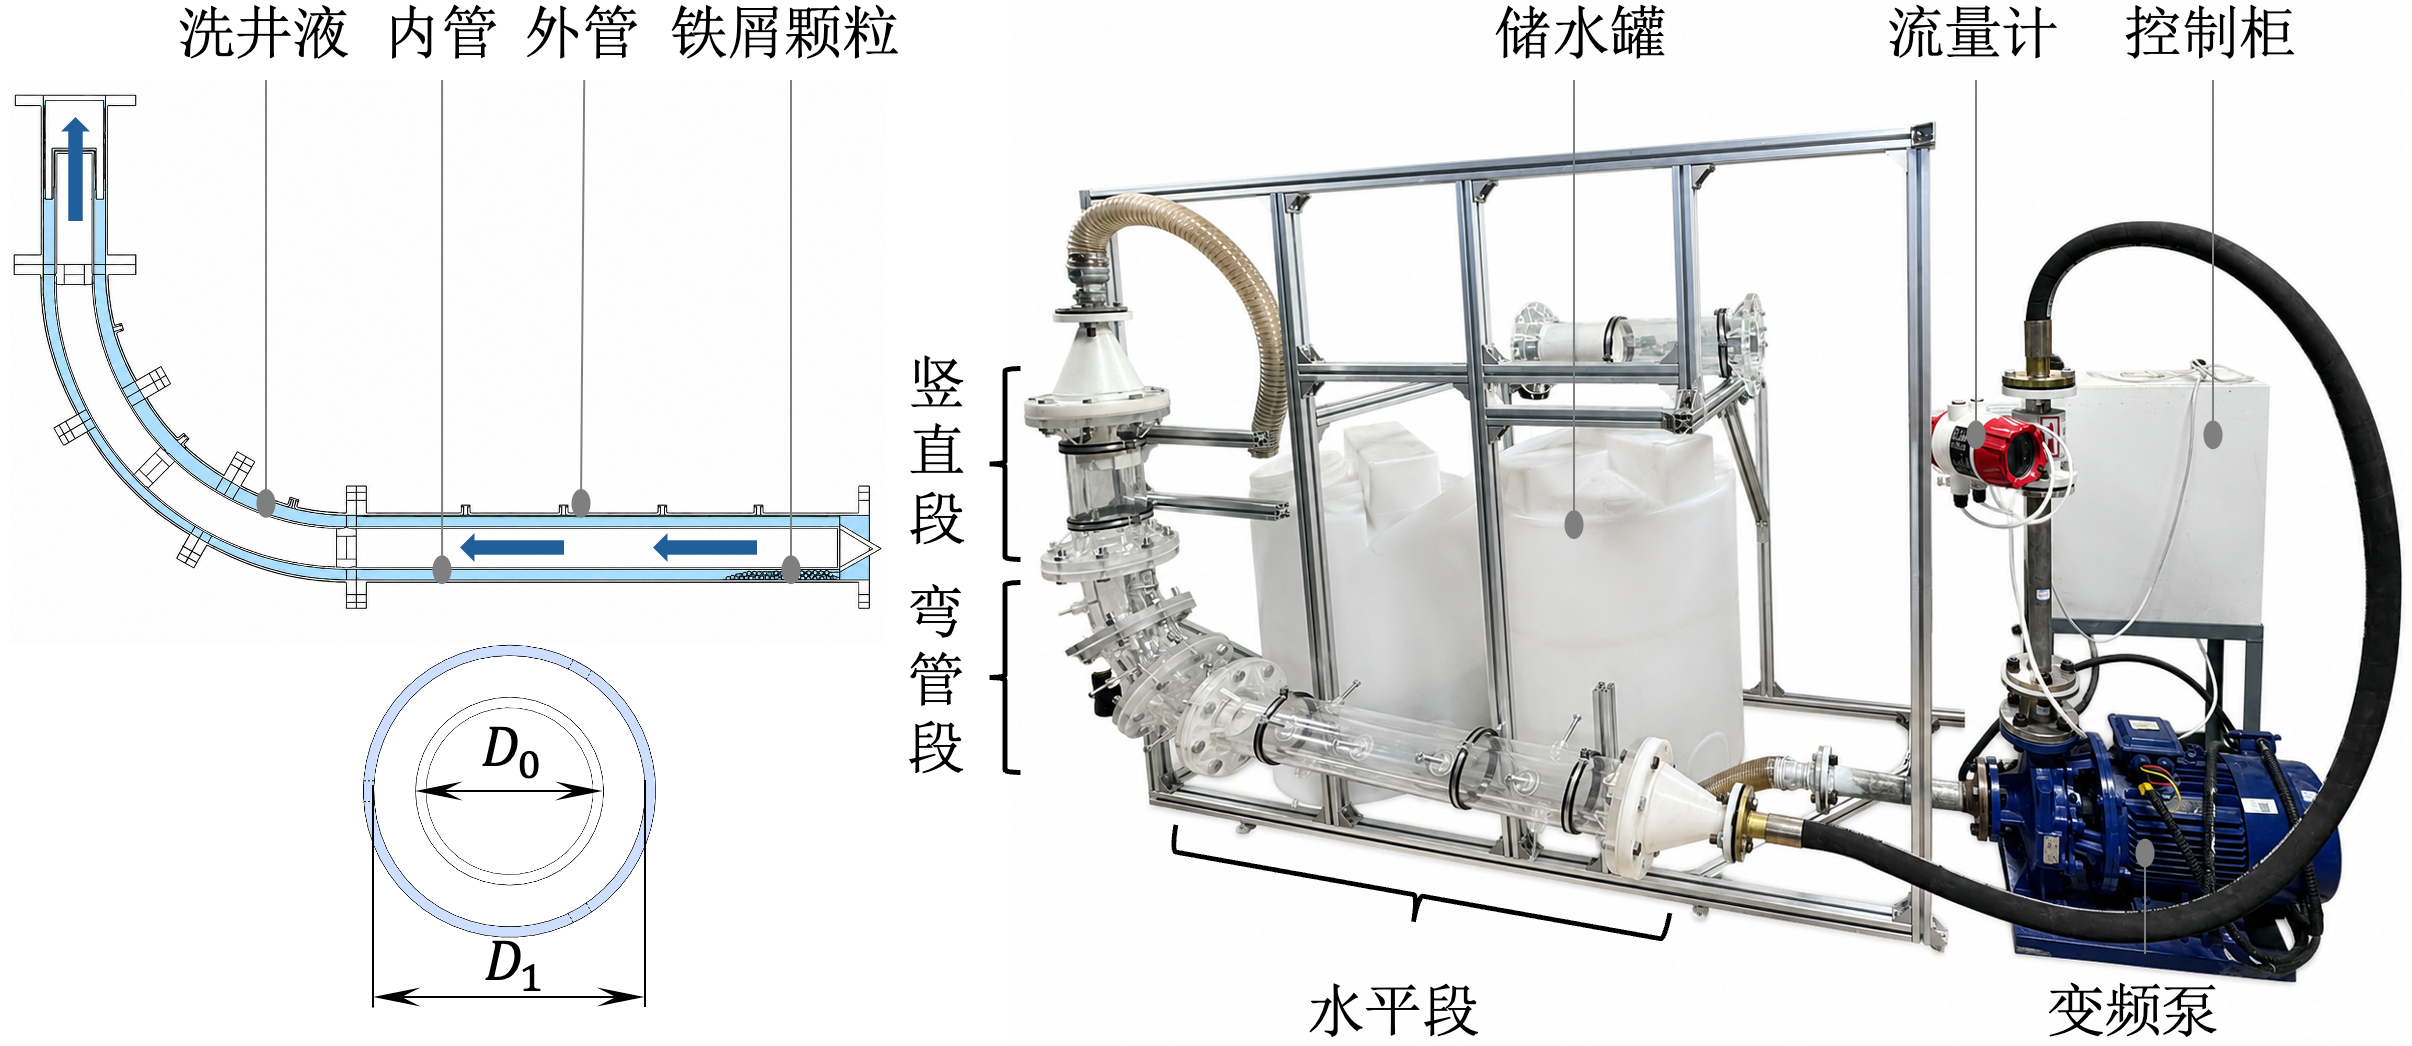
\includegraphics[width=1.\textwidth]{figure/chapter2/iron-washing-test-rig.png}
	\caption{研究洗井过程中铁屑运移规律的实验装置}
	\label{fig:iron_washing_test_rig}
\end{figure}

\subsection{实验结果及讨论}

水平段铁屑床的形态演变情况如图 \ref{fig:iron_bed_horizontal} 所示。随着泵流量$Q$的逐步增加，床层的宏观演化过程及流场特征表现出显著的阶段性规律。
当$Q=7.5\mathrm{m^3/h}$ 时，床层内的铁屑颗粒开始呈现运动趋势，部分颗粒自床层前缘起发生向后的位移，标志着床层由静止向流态化转变的初始阶段。当 $Q=10.00\mathrm{m^3/h}$ 时，铁屑床的宏观形态呈现出明显的非均匀拉伸特征：床层上部颗粒的运移距离显著大于下部颗粒。这种沿周向分布的运移差异表明，尽管设置了导流锥，但进口区域的流速分布不均现象尚未被完全消除，局部流场仍存在明显的梯度效应。
% TODO(核对): 正文 Q=7.5 m³/h 与图注 Q=7.85 m³/h 不一致，需以实测记录为准。
随着$Q=11.70\mathrm{m^3/h}$，铁屑床发生显著的宏观位移，其前缘已接近当前观测视野的边界。值得注意的是，在此高流量工况下，床层形态的演化反而表现出更高的均匀性与对称性。这一现象证实，随着流体向下游发展，环空区域的流速分布趋于均匀化，表明本实验系统对来流均匀性的整体控制质量良好，能够满足后续研究的流场要求。
\begin{figure}[htbp]
	\centering
	\subfloat[$Q=7.85\mathrm{m^3/h}$]{%
	
\includegraphics[width=.33\textwidth]{figure/chapter2/iron-bed-7dot85mperh.png}
	\label{fig:iron_bed_7dot85mperh}
	}
	%\vspace{1em}
	\subfloat[$Q=10.00\mathrm{m^3/h}$]{%
	
\includegraphics[width=.33\textwidth]{figure/chapter2/iron-bed-10dot00mperh.png}
	\label{fig:iron_bed_10dot00mperh}
	}
	\subfloat[$Q=11.70\mathrm{m^3/h}$]{%
	
\includegraphics[width=.33\textwidth]{figure/chapter2/iron-bed-11dot70mperh.png}
	\label{fig:iron_bed_11dot70_mperh}
	}
	\caption{水平段上铁屑床形态演变（铁屑床初始位置处俯视相机拍摄）}
	\label{fig:iron_bed_horizontal}
\end{figure}

随着流量的逐级提升，铁屑床表现出复杂的运动特征。即便在水平管段，颗粒床在达到临界启动流量后也非呈现简单的整体滑移模式，而是表现出“前缘不断剥蚀消失、后缘持续重塑堆积”的动态演化规律，且在整个运移过程中都有部分细小碎屑会受流体曳力作用从床层主体剥离，随主流场输运，导致铁屑床的质量递减。床层整体的运移速度随流速的增加而提升，但相对于环空的平均流速而言是较小值。弯管段与竖直段观测窗内的铁屑床形态演变分别如图\ref{fig:iron_bed_bend}和图\ref{fig:iron_bed_vertical}所示。
%后面的数据处理和速度为小值有直接关系，这里要扩展一下

\begin{figure}[htbp]
	\centering
	\subfloat[$Q=15.70\mathrm{m^3/h}$]{%
	
\includegraphics[width=.33\textwidth]{figure/chapter2/iron-bed-15dot70mperh.png}
	\label{fig:iron_bed_15dot70mperh}
	}
	%\vspace{1em}
	\subfloat[$Q=15.83\mathrm{m^3/h}$]{%
	
\includegraphics[width=.33\textwidth]{figure/chapter2/iron-bed-15dot83mperh.png}
	\label{fig:iron_bed_15dot83mperh}
	}
	\subfloat[$Q=17.44\mathrm{m^3/h}$]{%
	
\includegraphics[width=.33\textwidth]{figure/chapter2/iron-bed-17dot44mperh.png}
	\label{fig:iron_bed_17dot44_mperh}
	}
	\caption{弯管段铁屑床形态（弯管处正视相机拍摄）}
	\label{fig:iron_bed_bend}
\end{figure}

\begin{figure}[htbp]
	\centering
	\subfloat[铁屑床形态视频截图]{%
	
\includegraphics[width=.9\textwidth]{figure/chapter2/video-clip-theta-le-72-degree.png}
	\label{fig:video_clip_theta_le_72_degree}
	}
	\vspace{.5em}
	\subfloat[床面积提取结果]{%
	\begin{tikzpicture}
        % ================= 1. 放置完整的大图 =================
        % [name=img] 为图片命名，方便我们后续获取它的宽度
        % 替换 example-image 为你拼接好的那张完整大图的真实文件名（例如 full_image.png）
        \node[inner sep=0] (img) {
\includegraphics[width=.9\textwidth]{figure/chapter2/extraction-of-pack-area-theta-le-72-degree.png}};
        % ================= 2. 设置注释参数 =================
        % 这里的坐标是相对于大图的左下角 (0,0) 计算的
        \def\texty{-1.6} % 控制所有文字距离图片底部的垂直距离 (根据图片比例调整，负数表示向下偏移)
        % ================= 3. 在绝对坐标处添加注释 =================
        % 这里的 x 坐标（如 1.8, 3.6 等）是等间距的
        % 你需要根据你真实图片中子图的间距，手动微调这些 x 坐标
        \node at (-6.0, \texty) {${A^* = 1.00}$};
        \node at (-3., \texty) {${A^* = 0.64}$};
        \node at (0.0, \texty) {${A^* = 0.34}$};
        \node at (3., \texty) {${A^* = 0.05}$};
        \node at (6., \texty) {${A^* \approx 0.00}$};
    \end{tikzpicture}
	\label{fig:extraction_of_pack_area_theta_le_72_degree}
	}
	\caption{竖直段铁屑床形态（竖直管左视相机拍摄）}
	\label{fig:iron_bed_vertical}
\end{figure}

为精确量化这一过程，实验后通过视频帧分析提取了关键时间节点下的流量、位置及残留状态数据；特别是在弯管段的位置标定中，采用了实验视频与带刻度三维模型重叠匹配的方法，通过读取铁屑堆首尾端的刻度值，精确解算了床层质心的空间位置。实验观测表明，铁屑在弯管内的宏观迁移与进入竖直段后的流态化消散呈现出截然不同的动力学特征。前者主要体现为床层整体位置的时空演变，后者则侧重于固定堆积量的衰减过程。鉴于此，后续数据处理将针对这两个阶段分别选取特定的响应变量进行定量分析。

位置标定数据来自对原始视频的逐帧标定：在每个时刻识别铁屑床的头部与尾部，取二者角度的平均值作为床层中部位置，并记录对应的流量读数。标定共获得 $20$ 个有效点，如图\ref{fig:bed_position_VS_flow_rate_inclined_section}所示。角度范围覆盖 $\theta_c=0^{\circ}$-$72^{\circ}$，流量 $Q=14.25$-$18.09 \mathrm{m^3/h}$。其中 $\theta_c=51^{\circ}$-$63^{\circ}$区间因流量计读数在该时间段内出现异常波动，原始记录未采集到有效数据，这一区间在后续拟合中不参与计算，模型曲线由两侧的数据共同约束、连续给出。
$\theta_c>72^{\circ}$后，铁屑床主要进入竖直观察段并局部堆积，用弯管角度描述位置已不再适用，因此第二阶段改用视频提取的固定床可见面积作为响应量，用以描述床层的消散过程。

\begin{figure}[htbp]
	\centering
	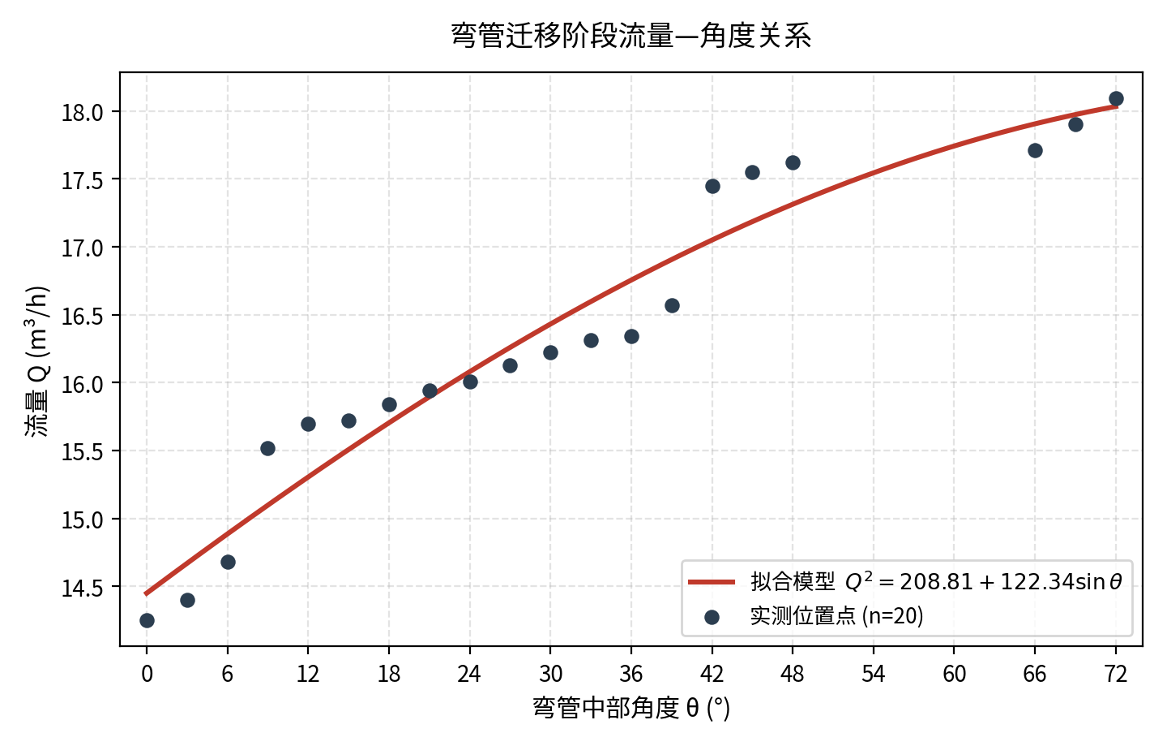
\includegraphics[width=1.0\textwidth]{figure/chapter2/bed-position-VS-flow-rate-inclined-section.png}
	\caption{弯管段铁屑床中部位置与流量的标定关系（$20$ 个有效标定点）}
	\label{fig:bed_position_VS_flow_rate_inclined_section}
\end{figure}
% TODO(待补): 给出各帧对应的流量/时刻与 A*(Q) 定量关系（第二阶段衰减模型），并与式\eqref{eq:bend_model}衔接。
在弯管迁移阶段，驱动铁屑床向前移动的是水流对床层的作用力，而阻碍其移动的主要是重力沿弯管切线方向的分量。参考直管水力学中过流量与壁面切应力的关系，流体作用力近似随流量的平方（$Q^2$）增长；重力切向分量则随弯管角度的正弦（$\sin\theta_c$）增长，在 $\theta_c=0^\circ$ 处最小、随角度增大而增大。将两者放在同一个力平衡框架下，可以得到如下候选形式
\begin{equation}
	Q^2(\theta_c) = A + B\cdot \sin\theta_c
	\label{eq:bend_candidate}
\end{equation}
式中，$A$、$B$为待定系数，量纲均为 $\mathrm{(m^3/h)^2}$。这一形式只用到了两个可从数据中辨识的组合参数，物理方向与力平衡机制一致，是后续候选模型比较的核心对象。

为避免主观选定单一形式，本文在同一数据集上比较了四类候选模型（见表\ref{tab:model_comparison}），统一以流量$Q$作为响应变量，通过决定系数$R^2$、均方根误差 RMSE、修正后的 AICc 以及留一交叉验证 RMSE（LOOCV RMSE）综合评估拟合优度与泛化能力：

\begin{table}[htbp]
    \centering
    \caption{候选模型拟合与交叉验证结果对比}
    \label{tab:model_comparison}
    \renewcommand{\arraystretch}{1.3}
    \begin{tabular}{llccccc}
        \toprule
        模型 & 函数形式 & 参数个数 & $R^2$ & RMSE & AICc & LOOCV RMSE \\
        \midrule
        重力分量力平衡 & $Q^2 = A + B\sin\theta_c$ & 2 & 0.942 & 0.267 & -48.15 & 0.294 \\
        二次多项式 & $Q = a + b\theta_c + c\theta_c^2$ & 3 & 0.943 & 0.265 & -45.63 & 0.302 \\
        经验幂函数 & $Q = Q_0 + c\theta_c^p$ & 3 & 0.945 & 0.261 & -46.26 & 0.313 \\
        线性 & $Q = a + b\theta_c$ & 2 & 0.911 & 0.331 & -39.50 & 0.376 \\
        \bottomrule
    \end{tabular}
\end{table}

二次多项式与经验幂函数的样本内 $R^2$ 略高于力平衡模型，但二者多用了一个自由参数，留一交叉验证误差反而没有改善，说明额外的自由度更多是在拟合噪声而非提升泛化能力。重力分量力平衡模型同时取得最低的 AICc 和最低的 LOOCV RMSE，且只用两个参数即达到与三参数模型相当的拟合优度，因此被选为最终模型。更高阶的分段拟合虽然可能进一步推高样本内 $R^2$ ，但会把 $\theta_c=51^\circ$～$63^\circ$ 的数据缺失和流量的局部波动误拟合成结构性拐点，不适合当前的数据规模。基于 $20$个有效位置点，最终确定的弯管迁移阶段模型为
\begin{equation}
	Q^2(\theta_c) = 208.57 + 122.69\sin \theta_c, \quad 0^\circ \le \theta_c \le 72^\circ
	\label{eq:bend_model}
\end{equation}
其中，基线项 $208.57$ 代表弯管起点附近床层接触、形状嵌锁与摩擦等综合阻力所对应的启动流量平方；系数 $122.69$ 代表重力切向分量随角度上升而增加的贡献。模型整体 $R^2$为 $0.942$，流量 RMSE 为 $0.267 \mathrm{m^3/h}$，LOOCV RMSE 为 $0.294 \mathrm{m^3/h}$。参数的 Bootstrap 95\% 置信区间为 $A \in [202.43, 216.75]$，$B \in [107.72, 134.89]$。由基线项换算得到的模型基准启动流量为 $Q_0 = 14.44 \mathrm{m^3/h}$（95\% 区间 $14.23-14.72 \mathrm{m^3/h}$），与实测中铁屑床到达弯管起始处的流量$14.25\mathrm{m^3/h}$ 十分接近，二者相互印证，说明模型在起点附近具有良好的物理合理性。
% TODO(待补): 补充 20 个标定点的数据表（或附录），以及 Bootstrap 重采样次数与置信区间方法说明。

因此，本文建立的是弯管迁移阶段的半经验模型与竖直段床层衰减的定量图像判据，用于描述本装置、本介质条件下铁屑床的启动、迁移与完全冲洗规律。


最终实验表明，随着泵流量增加，铁屑床经历由启动、沿弯管迁移、进入竖直段聚集并逐渐衰减，直至无可见颗粒的连续变化过程。在本实验条件下，约 $21.5\ \mathrm{m^3/h}$ 可作为最小观察性完全冲洗参考流量，约 $21.8\ \mathrm{m^3/h}$ 可作为较保守的无可见颗粒确认流量。
% TODO(待补): 说明 21.5 与 21.8 m³/h 的判定依据（无可见颗粒判据、观测窗分辨率），以及二者超出式\eqref{eq:bend_model}适用范围的说明。
需要说明的是，上述结论来源于本装置、本次约 $70\ \mathrm{g}$ 短小卷曲车削铁屑及当前流体条件下的一次连续升流量实验。由于流量与时间在实验中同步变化，且缺少多组恒定流量下的重复实验，所得模型与特征流量仅用于描述本台架条件下的实验规律；受数据规模与工况覆盖限制，尚不足以建立可外推至其他管径、流体或铁屑形态的完整输沙模型（如 Exner 输沙模型、Shields 临界起动模型或两层流模型），不宜直接外推至现场工况。

